%!TEX root = thesis.tex

\chapter{Visualisation Refinement}
\label{chap:visualisation-refinement}

\begin{chapquote}{Frederick Brooks, \textit{The Mythical Man-Month}}
``Geometric abstractions are powerful tools. The floor plan of a building helps both architect and client evaluate spaces, traffic flows, views. Contradictions become obvious, omissions can be caught. Scale drawings of mechanical parts and stick-figure models of molecules, although abstractions, serve the same purpose. A geometric reality is captured in a geometric abstraction.''
\end{chapquote}

Following the first user study (Chapter~\ref{chap:user-study}), limitations with both the visualisations and the evaluation method were identified and steps were taken to correct these limitations. The following section seeks to identify the steps taken to correct these limitations.

\section{Rationale}


``the aesthetic of fixing nodes and edges to an underlying unit grid was prominent''~\cite{Purchase2014} (also~\cite{Purchase2001,Purchase1996})

-previous study had some apparently conflicting results...
-previous study did not have a baseline - this was to be remedied
-previous study had visualisation limitations eg. missed timing, no direct feedback from the programmer etc


-strategy employed a combination of the aesthetic and didactic visualisations from the previous study...

\section{Design}

\cite{Purchase1996}...

\begin{figure}
  \centering 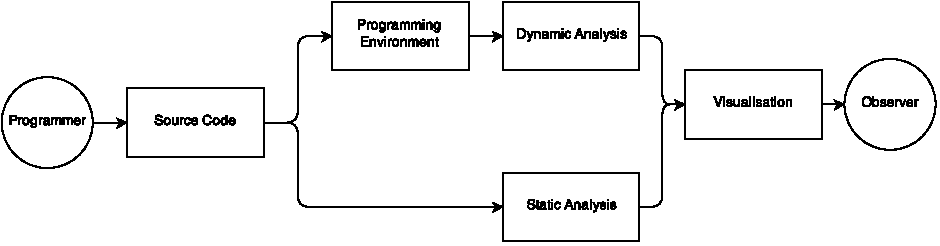
\includegraphics[width=\columnwidth]{../images/diagrams/knowledge-flow-refined.pdf}
  \caption{Knowledge flow from programmer to observer as directed by the visualisation technique employed.}
\label{fig:knowledge-flow-refined}
\end{figure}

\begin{figure}
  \centering 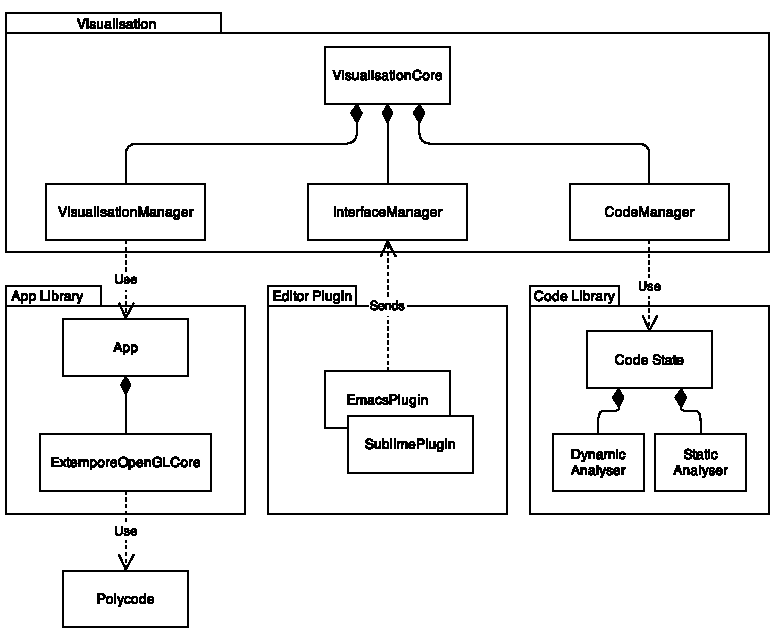
\includegraphics[width=\columnwidth]{../images/diagrams/visualisation-class-diagram.pdf}
  \caption{Class diagram of the visualisation technique employed.}
\label{fig:visualisation-class-diagram}
\end{figure}

The visualisation technique employed required three major components including an application manager, a code manager and an editor plugin (see the class diagram in Figure~\ref{fig:visualisation-class-diagram}). The following sections detail the implementation of these components.

\subsection{Visualisation Manager}

-polycode~\cite{Safrin2013}

-opengl

\subsection{Interface Mananger}
\label{sec:interface-manager}

-sublime plugin

-emacs plugin

This was acheived using a text editor plugin sending programmer interactions over an \ac{OSC} protocol. The interactions sent included cursor movement, all source code changes, file focus and source code evaluation.

\subsection{Code Manager}

Both static analysis of source code and the dynamic analysis (see the combined static and dynamic approach taken in~\cite{Eisenbarth2003}) of the running program were combined into this iteration of the visualisation prototype in order to provide the audience with a link between the \ac{SoW} and the \ac{SoC}~\cite{Swift2013}. {\color{red} explain what the \ac{SoW} and the \ac{SoC} actually is and show the link between the \ac{SoW} with dynamic analysis and the \ac{SoC} with static analysis...}

Static analysis of the source code involved parsing the changing source code input by the programmer. Data requiring this static analysis was received from the editor plugin (see~\ref{sec:interface-manager}) and stored as the current \ac{SoC}.

Dynamic analysis of the running program involved providing mechanisms for the programmer to send running state information to be stored as the \ac{SoW}. {\color{red} explain what was provided a little better} A callback hook was provided to be used when creating an instrument during performance. This hook would provide data on the state of the active instruments and would allow links to be determined between the \ac{SoC} and the \ac{SoW}.

\subsection{Mappings}

A number of specific mappings were assigned to the visualisation. These visual mappings related directly to actions taken by the programmer. 

-function count
-function active/inactive state
-function size/shape
-function beat+callback duration
-programmer editing behaviour
-programmer typing behaviour

{\color{red} Show a table with images and description of behaviour}

\section{Summary}

-how does this visualisation fix the issues identified in the previous iteration of the visualisation?



